\documentclass[a4paper, 11pt]{book}

\newcommand*{\plogo}{\fbox{$\mathcal{DB}$}}

\usepackage[utf8]{inputenc}
\usepackage{stix}
\usepackage[english]{babel}
\usepackage{amsfonts}
\usepackage{amsthm}
\usepackage{amsmath}
\usepackage{amssymb}
\usepackage{nicefrac}
\usepackage{commath}
\usepackage{dirtytalk}
\usepackage{tikz-cd}

\usepackage{graphicx}

\newtheorem{theorem}{Theorem}
\newtheorem{es}{Examples}
\newtheorem*{example}{Example}

\newcommand\restr[2]{{% we make the whole thing an ordinary symbol
    \left.\kern-\nulldelimiterspace % automatically resize the bar with \right
    #1 % the function
    \vphantom{\big|} % pretend it's a little taller at normal size
    \right|_{#2} % this is the delimiter
}}

\theoremstyle{definition}
\newtheorem{definition}{Definition}[section]
 
\theoremstyle{remark}
\newtheorem*{remark}{Remark}

\newtheorem{corollary}{Corollary}[theorem]
\newtheorem{lemma}[theorem]{Lemma}

\newtheorem{prop}{Proposition}

\newcommand{\inter}[1]{int(#1)}

\begin{document}

    \begin{titlepage} 
        \raggedleft

        \rule{1pt}{\textheight} % Vertical line
        \hspace{0.05\textwidth} % Whitespace between the vertical line and title page text
        \parbox[b]{0.75\textwidth}{ % Paragraph box for holding the title page text, adjust the width to move the title page 
            % left or right on the page
                            
            {\Huge\bfseries MAT1847 Lecture \\[0.5\baselineskip] Notes }\\[2\baselineskip] % Title
            {\large\textit{Lecture notes on a course Holomorphic Dynamics}}\\[4\baselineskip] % Subtitle or further description
            {\Large\textsc{A. Wortschöpfer}} % Author name, lower case for consistent small caps
                                                    
            \vspace{0.5\textheight} % Whitespace between the title block and the publisher
                                                            
            {\noindent The Publisher~~\plogo}\\[\baselineskip] % Publisher and logo
        }
    \end{titlepage}

    \chapter{Riemann Surfaces}

    The next three sections are meant to be an overview of background material required for this course.

    \section{Simply Connected Surfaces}

    \begin{definition}[Riemann Surface]
        A \textbf{Riemann surface} is a connected, paracompact, Hausdorff topological space $X$ equipped with an open covering $\{U_i\}$ 
        and a collection of homeomorphisms $f_i: U_i\to\mathbb{C}$ such that there exist analytic (i.e. holomorphic) $g_{ij}$ 
        such that
        \[ f_i \circ f_j^{-1} = g_{ij} \]
        where we have the assumption $U_i\cap U_j\neq 0$. We refer to the collection $\{(U_i,f_i)\}$ as the \textbf{chart} of 
        the Riemann surface. An equivalent way defining a Riemann surface is as follows:
        A Riemann surface is a connected complex analytic manifold of complex dimension 1.
    \end{definition}

    \begin{example}
        The complex plane $\mathbb{C}$ is the most basic Riemann surface. $\mathbb{C}$ is not only connected but also
        \textit{simply} connected and is also clearly Hausdorff and paracompact. The chart is given by $\{(\mathbb{C},i)\}$
        where $i: \mathbb{C}\to\mathbb{C}$ is the identity function. In fact, any non-empty open set $U$ of $\mathbb{C}$ (for example
        $\mathbb{H} = \{z\in\mathbb{C}: $Im$(z)>0\}$) is also a Riemann surface.
    \end{example}

    \begin{example}[Riemann sphere]
        The Riemann sphere is another example of a \textit{simply} connected Riemann surface. This sphere is not a subset
        of $\mathbb{C}$ nor is it biholomorphic to $\mathbb{C}$. This is the extended complex plane (i.e. $\mathbb{C}\cup\{\pm\infty\}$).
        Geometrically, this can be idealized using \textit{stereographic projection}:\\
        Identify the $xy-$plane (in $\mathbb{R}^3$) with $\mathbb{C}$. Let $\mathbb{S}$ be the sphere sitting in $\mathbb{R}^3$ centered
        at $(0,0,\nicefrac{1}{2})$ and of radius $\nicefrac{1}{2}$. Also, denote $\mathbb{N}$ to be the North pole of $\mathbb{S}$.
        Then, given any point $W = (X,Y,Z)$ on $\mathbb{S}-\mathbb{N}$, the line joining $N$ and $W$ intersects the $xy$-plane at
        a single point $w$. We say that $w$ is the \textbf{stereographic projection} of $W$. The inverse map can also be derived
        similarly, therefore we have a bijective mapping between $\mathbb{S}-\mathbb{N}$ and $\mathbb{C}$. As the point $w$ goes to
        infinity in $\mathbb{C}$ (i.e. $|w|\to\infty$) the corresponding point $W$ on $\mathbb{S}$ comes arbitrarily close to 
        $\mathbb{N}$. Thus, we can define $\mathbb{N}$ to be the point at infinity. Therefore, we can identify the extended complex 
        plane with the sphere $\mathbb{S}$.
    \end{example}

    \begin{remark}
        We can show that the projection mapping is not only a bijective mapping but a \textit{diffeomorphic} mapping. This makes
        showing that transition maps are holomorphic not too hard.
    \end{remark}

    \begin{definition}[Conformal]
        A function $f:\mathbb{C}\to\mathbb{C}$ is \textbf{conformal} if it preserves angles.
    \end{definition}

    \begin{remark}
        A function $f:\mathbb{U}\to\mathbb{C}$ is \textbf{holomorphic} if
        \begin{enumerate}
            \item the Cauchy-Riemann equations hold i.e.
                \[ \overline{\partial}{f} = 0\qquad\text{and}\qquad \nicefrac{\partial{f}}{\partial{\overline{z}}} = 0 \]
            \item \[ \lim_{h\to 0} \frac{f(z+h)-f(z)}{h} = f'(z)\quad\text{exists} \]
            \item For all $z_0\in U$, there exists a convergent power series such that $f(z) = \sum_{n=0}^{\infty} a_nz^n$ for
                $z$ in a neighbourhood of $z_0$.
        \end{enumerate}
    \end{remark}

    \begin{remark}
        A holomorphic function $f:V\to\mathbb{C}$ is \textbf{conformal} if the derivative $f'(z)$ never vanishes i.e. $f'(z_0)\neq 0$
        for all $z\in V$. (note $f': V\to\mathbb{C}$ also and $f'(z)\neq 0$ implies that $f$ is locally injective). We can see this
        through:
        \begin{align*}
            f'(z_0) &= \lim_{h\to0} \frac{f(z+h)-f(z)}{h} \\
            \implies f(z+h) &\approx f(z) + f'(z)h
        \end{align*}
        Recall that multiplying by a number (non-zero and complex) is a composition of rotation and dilation so $f$ is conformal.
    \end{remark}

    There are three main \textit{simply} connected Riemann surfaces that are distinct (general case is uncountable).

    \begin{theorem}[Uniformization Theorem]
        Any simply connected Riemann surface is conformally isomorphic either
        \begin{enumerate}
            \item to the open disk $\mathbb{D}\subset\mathbb{C}$ consisting of all $|z|^2 < 1$ or,
            \item to the plane $\mathbb{C}$
            \item to the Riemann sphere $\hat{\mathbb{C}}$
        \end{enumerate}
    \end{theorem}

    To see that these are indeed inequivalent surfaces, we have to talk about the following:

    \begin{theorem}[Liouville]
        Every entire, bounded function is constant.
    \end{theorem}

    \begin{corollary}
        $\mathbb{C}$ is not biholomorphic to $\mathbb{D}$.
    \end{corollary}
    \begin{proof}
        Let $f$ be a holomorphic function $f:\mathbb{C}\to\mathbb{D}$. Then, $f$ is bounded since $D$ is bounded. By Liouville's
        theorem, we have that $f$ is constant. Since constant functions are clearly not bijective, we have that $f$ is not
        biholomorphic. Therefore, there exist no biholomorphic maps between $\mathbb{C}$ and $\mathbb{D}$. 
    \end{proof}

    It is clear that $\hat{\mathbb{C}}$ is not biholomorphic to any of the other Riemann surfaces on the list above since it is
    compact and the two other surfaces are not. Here is another way to arrive at the same conclusion:

    \begin{remark}
        There are no non-constant biholomorphic maps $f:\hat{\mathbb{C}}\to\mathbb{C}$.
    \end{remark}
    \begin{proof}
        It is clear that $f(\hat{\mathbb{C}})$ is compact since $\hat{\mathbb{C}}$ is and $f$ is continuous. By the open mapping
        theorem, if $f$ is non-constant, $f(\hat{\mathbb{C}})$ is open. However, there are no open compact subsets of $\mathbb{C}$.
        Therefore, $f$ is constant as wanted.
    \end{proof}

    \begin{remark}
        $\mathbb{D}\hookrightarrow \mathbb{C} \hookrightarrow \hat{\mathbb{C}}$.
    \end{remark}

    \begin{corollary}
        Every Riemann surface is the quotient of either $\mathbb{D},\mathbb{C}$, or $\hat{\mathbb{C}}$ by a discrete group $\Gamma$
        of automorphisms of $\mathbb{D},\mathbb{C},$ or $\hat{\mathbb{C}}$.
    \end{corollary}

    To prove this, we recall several algebraic and topological notions.

    \begin{definition}
        A map $p: M\to N$ between connected manifolds is a \textbf{covering map} if every point of $N$ has a connected open
        neighborhood $U$ within $N$ which is \textbf{evenly covered}; that is, each component $p^{-1}(U)$ must map onto $U$
        by a homeomorphism. The manifold $N$ is \textbf{simply connected} if it has no nontrivial coverings, that is, if every
        such covering map $M \to N$ is a homeomorphism. For any connected manifold $N$, there exists a covering map $\widetilde{N}
        \to N$ such that $\widetilde{N}$ is simply connected. This is called the \textbf{universal covering} of $N$ and is
        unique up to the homeomorphism. By a \textbf{deck transformation} associated with a covering map $p: M\to N$ we mean
        a continuous map $\gamma:M\to M$ which satisfies the identity $p\:\circ\:\gamma = p$, so that the diagram
        \begin{equation*}
        \begin{tikzcd}
            M \arrow[rr, "\gamma"] \arrow[dr, "p",swap]&  & M\arrow[dl, "p"]\\ 
            & N &
        \end{tikzcd}
        \end{equation*}
        is commutative.
    \end{definition}

    \newpage

    \begin{definition}
        For our purposes, the \textbf{fundamental group} $\pi_1(N)$ can be defined as the group $\Gamma$ consisting of all deck
        transformations for the universal covering $\widetilde{N}\to N$. Note that this universal covering is always a 
        \textbf{normal covering} of $N$. That is, given two points $x,x'\in M = \widetilde{N}$ with $p(x)=p(x')$, there exists
        and only one deck transformation which maps $x$ to $x'$.
    \end{definition}

    It follows that $N$ can be identified with the quotient $\nicefrac{\widetilde{N}}{\Gamma}$ of $\widetilde{N}$ by this action
    of $\Gamma$. We are finally ready to now prove the aforementioned corollary.

    \begin{proof}
        $X$ is a Riemann surface, then $\widetilde{X}$ (universal cover of $X$) is also a Riemann surface and furthermore,
        it is also simply connected. Hence,
        \[ X \simeq \frac{\widetilde{X}}{\Gamma} \]
        where $\nicefrac{\widetilde{X}}{\Gamma}$ is the collection of equivalence classes given by the relation $x\sim y$ if there
        exists $\gamma\in\Gamma$ such that $\gamma(x) = y$. Furthermore, if $x\sim y$ is given, then $p(x) = p(\gamma(x)) = p(y)$
        by definition of a deck transformation. Therefore, we have an identification $[x]\mapsto p(x)$. Finally, it is clear that
        $\Gamma <\: $Aut$(\widetilde{X})$ (i.e. $\Gamma$ is a subset of...)
    \end{proof}

    Using the corollary above, we can define the following:

    \begin{definition}
        A Riemann surface $X$ is called:
        \begin{enumerate}
            \item \textbf{elliptic} if $\widetilde{X} = \hat{\mathbb{C}}$ (in fact, if $\widetilde{X} = \hat{\mathbb{C}}$, then
                $X = \hat{\mathbb{C}}$,
            \item \textbf{parabolic} or sometimes \textit{flat} if $\widetilde{X} = \mathbb{C}$,
            \item \textbf{hyperbolic} if $\widetilde{X} = \mathbb{D}$
        \end{enumerate}
    \end{definition}

    We now study the spaces of all biholomorphic maps $X\to X$ ($X$ a Riemann surface). By the corollary above, we see that it
    suffices to study only the three simply connected Riemann surfaces. Denoting the set of all biholomorphic maps from $X\to X$ by
    Aut$(X)$, we are then studying the spaces: Aut$(\hat{\mathbb{C}})$, Aut$(\mathbb{D})$ and Aut$(\mathbb{C})$.\\

    We begin by studying Aut$(\hat{\mathbb{C}})$.

    \begin{theorem}
        Aut$(\hat{\mathbb{C}}) = \{$Möbius transformations$\} = \{g: g(z) = \nicefrac{az+b}{cz+d}\}$ where the coefficients are
        complex numbers with $ad-bc\neq 0$.
    \end{theorem}

    Note we can always normalize the $\nicefrac{az+b}{cz+d}$ always so that the determinant of its associated matrix
    is +1 where the resulting coefficients are well defined up to simultaenous change of sign. Therefore, Aut$(X)$ can
    be identified with the Lie group $\mathbb{PSL}_2(\mathbb{C})$ consisting of $2 \times 2$ complex matrices with determinant
    1 modulo the subgroup $\{\pm I\}$.

    \begin{proof}
        The $\implies$ direction follows from the fact that each Möbius transformation is a biholomorphic map. For the other
        direction. Now take some $f\in$ Aut$(\hat{\mathbb{C}})$ and compose it with some Möbius transformtion (already proven
        to be a subset (in fact a subgroup) of Aut$(\hat{\mathbb{C}})$) so that we may assume $f(0) = 0$ and $f(\infty) = \infty$.
        Setting $z=e^w$, it follows that the composition $w\mapsto \nicefrac{f(e^w)}{e^w}$ is a bounded holomorphic function on
        $\mathbb{C}$. Hence it takes a constant value $c$ by Liouville's Theorem. Therefore $f(z)=cw$ is linear and hence $f$
        itself an element of $\mathbb{PSL}_2(\mathbb{C})$.
    \end{proof}

    \begin{remark}
        Every Möbius transformation has 2 fixed points in $\mathbb{C}$
        \[ z = \nicefrac{az+b}{cz+d},\qquad cz^2 + (d-a)z - b = 0 \]
        This implies that there is always at least one fixed point. If $\Gamma <$ Aut$(\hat{\mathbb{C}})$ is the deck group
        then any element has no fixed point so you must have $\Gamma = \{ I \}$.
    \end{remark}

    Now, we discuss what happens in the parabolic case.

    $\Gamma <$ Aut$(\mathbb{C}) = \{z\mapsto az+b: a,b\in\mathbb{C}, a\neq 0\} = \{\text{affine transformations}\}$.
    In fact, if $a=1$, then
    \[ z = az+b \]
    has a fixed point unless $a=1$. So,
    \begin{align*}
        \Gamma &< \{z\mapsto z+b, b\in\mathbb{C}\} \\
        \Gamma &= \{I\} \\
        \Gamma &= \{I, z\mapsto z+1\}
    \end{align*}
    where then $X = \nicefrac{\mathbb{C}}{\mathbb{Z}}\simeq \mathbb{C}-\{0\}$ is the cylinder where the $\simeq$ is seen by
    \[ g(z) = e^{2\pi iz},\;g:\mathbb{C}\to\mathbb{C}-\{0\},\; g(z+1) = g(z) \]
    (Note translations preserve the Euclidean metric which has $K=0$ so the cylinder is flat)\\
    For the other cases $\mathbb{D}-\{0\}$ and $A_r = \{1<|z|<R\}$, you have two translations,
    \[ \Gamma = \langle z\mapsto z+1,z\mapsto z+\tau\rangle \]
    \[ X = \nicefrac{\mathbb{C}}{\Gamma} = \{\text{the one-holed taurus}\} \]
    Thus for each $\tau\in\mathbb{H}$ (upper half plane of $\mathbb{C}$), you get $X_{\tau} = 
    \nicefrac{\mathbb{C}}{\mathbb{Z}+\mathbb{Z}\tau}.$\\

    If $\tau' = g(\tau)$ where $g\in\mathbb{SL}_2(\mathbb{Z})$ (special linear group), then
    \[ X_{\tau'} \simeq X_{\tau} \]
    So,
    \begin{align*}
        \wedge_{\tau} &= \mathbb{Z} + \mathbb{Z}_{\tau} \\
        g(\wedge_{\tau}) &= \wedge_{\tau}\qquad\text{if}\qquad g\in\mathbb{SL}_2(\mathbb{Z})
    \end{align*}

    Thus far, we have discussed the Automorphism groups of:
    \begin{enumerate}
        \item elliptic: $X = \hat{\mathbb{C}},\;$ Aut$(\hat{\mathbb{C}}) = \mathbb{PSL}_2(\mathbb{C})$.
        \item parabolic (flat): $X = \mathbb{C},\; \nicefrac{C}{\mathbb{Z}} \simeq \mathbb{C}-\{0\},\; 
                \nicefrac{C}{\mathbb{Z}+\mathbb{Z}\tau}$
    \end{enumerate}
    It is left to discuss the hyperbolic case i.e. when the curvature is $K = -1$ (in the elliptic case it was $K=1$ and $K=0$
    in the flat case).\\

    First, we show that there is a hyperbolic holomorphism between $\mathbb{D}$ and $\mathbb{H}$ by explicitly constructing one.
    Claim that it is given by
    \[ \mathbb{H}\to \mathbb{D},\qquad z\mapsto \frac{z-c}{z+c} \]
    Therefore, it suffices to find Aut$(\mathbb{H})$ since from above it follows Aut$(\mathbb{H})=$ Aut$(\mathbb{D})$\\
    Claim:
    \[ \text{Aut}(\mathbb{H}) = \{z\mapsto\frac{az+b}{cz+d}: a,b,c,d\in\mathbb{R}, ad-bc=1\} \simeq \mathbb{PSL}_2(\mathbb{R}) \]
    \begin{proof}
        Choose $g\in\mathbb{PSL}_2(\mathbb{R})$ so $g(\mathbb{H})\subseteq \mathbb{H}$. Note:
        \begin{align*}
            \text{Im}(\frac{az+b}{cd+d}) &=\:\text{Im}(\frac{(az+b)(c\overline{z}+d)}{|cz+d|^2} \\
            &= \text{Im}(\frac{a|z|^2+bd+adz+bc\overline{z}}{|cz+d|^2}) \\
            &= \frac{ad\text{Im}(z)-bc\text{Im}(z)}{|cz+d|^2} = \frac{\text{Im}(z)}{|cz+d|^2} > 0
        \end{align*}
    \end{proof}

    Why aren't there any others?
    \begin{proof}
        For any $z\in\mathbb{H}$, there is $g\in\mathbb{PSL}_2(\mathbb{R})$ such that $g(z) = i$.\\
        Given $g\in$ Aut$(\mathbb{H})$ such that $g(i) = i$, is $g\in\mathbb{PSL}_2(\mathbb{R})$?
    \end{proof}

    Now, we recall:
    \begin{lemma}[Schwarz Lemma]
        If $g:\mathbb{D}\to\mathbb{D}$ is holomorphic and $g(0)=0$, then $|g(z)| \leq |z|$ for any $z\in\mathbb{D}$ and if
        there exists $z\neq 0$ with $|g(z)|=|z|$, then:
        \[ \exists\; \theta\;\text{such that}\; g(z) = e^{i\theta}z \]
    \end{lemma}

    We can interpret this to mean that if $g$ preserves norm, it is a rotation, otherwise it retracts

    \begin{proof}
        $f(z) = \nicefrac{g(z)}{z}$ is holomorphic. Hence by maxmium principle, if $|z|\leq r<1$,
        \[ |f(z)| \leq\:\text{max}_{|z|=r} |f(z)| \leq \nicefrac{1}{r} \to 1 \]
        By maximum principle, if there exists $z$ such that $|\nicefrac{f(z)}{z} = 1$, then
        \[ \nicefrac{f(z)}{z} = c = e^{i\theta} \]
    \end{proof}

    \begin{corollary}
        If $g:\mathbb{D}\to\mathbb{D}$, $g(0)=0$, then $|g'(0)|\leq 1$. If $|g'(0)|=1$, then $g$ is a rotation.
    \end{corollary}

    \begin{corollary}
        If $g\in$ Aut$(\mathbb{D})$ and $g(0)=0$, then $g(z) = e^{i\theta}z$.
    \end{corollary}
    \begin{proof}
        Choose $g\in$ Aut$(\mathbb{D})$, then there exists $h$ such that $g\circ h =$ id.
    \end{proof}

    Given $g\in$ Aut$(\mathbb{H})$ such that $g(i) = i$, then
    \[ g(z) = \frac{z\cos{\theta}+\sin{\theta}}{-z\sin{\theta}+\cos{\theta}} \]
    For example, $\theta = \nicefrac{\pi}{2}$, then $g(z) = -\nicefrac{1}{z}$. On the Hyperbolic plane, one can imagine
    such mappings $g$ as a rotation around $z=i$.\\

    Thus,
    \begin{align*}
        \text{Aut}(\mathbb{H}) &= \{z\mapsto \frac{az+b}{cz+d}:a,b,c,d\in\mathbb{R},ad-bc=1\} \\
        \text{Aut}(\mathbb{D}) &= \{z\mapsto e^{i\theta}\frac{z-a}{1-z\overline{a}},|a|<1,0\leq\theta<2\pi\}
    \end{align*}
    Note, if $f(z) = \nicefrac{z-a}{1-z\overline{a}}$, then $f(f(z)) = z$.\\

    \section{Hyperbolic Metric}

    \begin{theorem}
        There exists up to scaling, a \textit{unique} Riemann metric on $\mathbb{H}$ (or $\mathbb{D}$) which is invariant by 
        Aut$(\mathbb{H})$. In formulas, it is given by:
        \[ ds = \frac{dz}{y} \]
        where $dz$ is the Euclidean metric and $y$ is the imaginary point.
    \end{theorem}

    In the Hyperbolic plane, we can imagine the distance between two points connected by a horizontal line becoming very big
    as it (the horizontal line) approaches Im$(z) = 0$ and very small as it moves away.\\

    The mapping
    \[ z\mapsto z+1 \]
    preserves $ds$. The mapping
    \[ z\mapsto \lambda z \]
    preserves $ds$ if $\lambda>1$.\\

    For $\mathbb{D}$, the Hyperbolic metric is given by
    \[ ds = \frac{2dz}{1-|z|^2} \]
    We want to normalize this so $K=-1$.

    \begin{remark}
        If $U\subsetneq \mathbb{C}$ is open, simply connected, there exists a biholomorphic mapping
        \[ f: U\to \mathbb{D} \]
        which defines the \textbf{hyperbolic metric} (Poincaré metric) on $U$
        \[ \rho_U = f_{\rho_\mathbb{D}} \]
        so,
        \[ ds_U \approx \frac{dz}{d(z,\partial U}) \]
    \end{remark}

    \section{Hyperbolic Riemann surfaces}

    Recall the classifications of Riemann surfaces:
    \[ X = \frac{\widetilde{X}}{\Gamma},\qquad \Gamma <\:\text{Aut}(\widetilde{X}),\qquad \widetilde{X} = \hat{\mathbb{C}},\mathbb{C},
        \mathbb{D}\simeq \mathbb{H} \]
    where $\Gamma$ is discrete torsion free. In the elliptic case (spherical, positive $K$):
    \[ \text{Aut}(X) = \mathbb{C} \]
    In the parabolic case (i.e. Euclidean/flat with $K=0$), we have
    \[ X = \mathbb{C},\nicefrac{\mathbb{C}}{\mathbb{Z}},\nicefrac{\mathbb{C}}{\wedge} \]

    We have the following \textit{fact}: If $X$ is a Riemann surfaces and $X\neq\hat{\mathbb{C}},\mathbb{C},\mathbb{C}-\{0\},
    \nicefrac{\mathbb{C}}{\wedge}$, then $\widetilde{X} = \mathbb{H}$. Note $\wedge =$ torus, $\mathbb{Z} + \mathbb{Z}\tau$.\\

    \begin{corollary}
        A Riemann surface $X$ such that $\widetilde{X} \simeq \mathbb{H}$ is called \textbf{Hyperbolic} and it carries a natural
        metric $\rho$ of constant negative curvature. This is called the \textbf{Poincaré metric}.
    \end{corollary}

    \begin{theorem}
        The upper half plane $\mathbb{H}$ carries a unique, up to scaling, Riemannian metric which is invariant by
        \[ \text{Aut}(\mathbb{H}) \simeq \mathbb{PSL}_2(\mathbb{R}) \]
    \end{theorem}

    First, we prove the corollary.

    \begin{proof}
        Note, $X \simeq \nicefrac{\widetilde{X}}{\Gamma} \simeq \nicefrac{\mathbb{H}}{\Gamma}$.\\
        Since The Hyperbolic metric is $\Gamma$-invariant, it defines a metric on $\widetilde{X} = \nicefrac{\mathbb{H}}{\Gamma}$.
    \end{proof}

    Before we prove the theorem, we remark:
    \begin{remark}
        In general, a Riemannian metric is given by
        \[ ds^2 = g_{11}dx^2 + 2g_{12}dxdy + g_{22}dy^2 \]
        A \textbf{conformal} metric on $X$ is given by
        \[ ds = \rho(z)dz \]
        where $\rho: X\to\mathbb{R}^{\geq 0}$ (Hyperbolic metric is conformal).
    \end{remark}

    \begin{proof}
        Note, $y =$ Im$(z)$ and $\rho = \nicefrac{|dz|}{y}$.\\
        Look at $g(z) = \nicefrac{az+b}{cz+d}$ for $a,b,c,d\in\mathbb{R}$:
        \[ g'(z) = \frac{[a(cz+d)-c(az+b)]}{(cz+d)^2} = \frac{ad-bc}{(cz+d)^2} = \frac{1}{(cz+d)^2} \]
        and,
        \begin{align*}
            \text{Im}(g(z)) =\:\text{Im}(\frac{az+b}{cz+d}) &=\:\text{Im}(\frac{(az+b)(c\overline{z}+d)}{|cz+d|^2}) \\
            &=\:\text{Im}(\frac{bc\overline{z}+adz}{|cz+d|^2}) = \frac{bc}{|cz+d|^2}\text{Im}(\overline{z}) + 
                \frac{ad\text{Im}(z)}{|cz+a|^2} \\
            &= \frac{\text{Im}(z)}{|cz+d|^2}
        \end{align*}
        So,
        \[ z' = g(z),\quad |dz| = |g'(z)|dz,\quad \frac{|dz|}{y'} = \frac{|g'(z)||dz|}{\text{Im}(g(z))} = \frac{dz}{\text{Im}(z)} \]
        For uniqueness:\\
        Suppose the conformal metric $\rho(z)dz$ is $\mathbb{PSL}_2(\mathbb{R})$-invariant. Then, it is invariant by $f(z)=bz+a$
        so,
        \[ z' = f(z) \qquad \rho(z')dz' = \rho(f(z))|f'(z)|dz \stackrel{?}{=} \rho(z)dz \]
        Note, at $z=i$:
        \[ \rho(f(z)) = \frac{\rho(z)}{|f'(z)|},\qquad \rho(a+ib) = \frac{\rho(i)}{b} \]
        Hence, if we normalize so that $\rho(i) = i$, then $\rho(z) = \nicefrac{1}{\rho(\text{Im}(z))}$.\\

        What if it is not conformal?\\
        A Riemannian metric on $\mathbb{H}$ which is invariant must, by Aut$(\mathbb{H})$, be conformal. Note,
        \[ g(z) = \frac{\cos({\theta})z-\sin{\theta}}{z\sin{\theta}+\cos{\theta}} \]
        rotates around $z=i$. More percisely, $g(i) = i$, and $dg_i$ acts as a rotation aon $T_i(\mathbb{H})$ (tangent plane).\\
        Hence the metric induced by $\rho$ on $T_i(\mathbb{H})$ is a multiple of the Euclidean metric since it is rotationally invariant.
    \end{proof}

    \begin{lemma}
        The disk $\mathbb{D}$ with the Hyperbolic metric is \textbf{complete}. Moreover, any path leading from $z_0\in\mathbb{D}$ to 
        a point $\partial{\mathbb{D}}$ has infinite length. Any two points of $\mathbb{D}$ one joined by unique geodesics of minimal
        length.\\
        In the disk model, geodesics are arcs of circles which are orthogonal to $\partial{\mathbb{D}}$.
    \end{lemma}
    \begin{proof}
        Take $\mathbb{H}$ as model.\\
        Note, given $z_1,z_2$ acting on Aut$(\mathbb{H})$, you can assume
        \[ \text{Re}(z_1) =\:\text{Re}(z_2). \]
        In the case of the vertical geodesic (the shortest line connecting two points is a vertical, straight line), we have
        \[ \rho = \frac{|dz|}{y},\qquad ds^2 = \frac{dx^2+dy^2}{y^2} \]
        So, the projection any path $\gamma$ between $z_1,z_2$ of $[z_1,z_2]$ is shorter. The lenght is,
        \[ d_{\mathbb{H}}(z_1,z_2) = \int_{y_1}^{y_2} \frac{1}{y}dy = \log{\frac{z_2}{z_1}},\qquad y_i =\:\text{Im}(z_i) \]
        The other case occurs when the geodesic between two points is an arc segment.\\
        Why is it complete?\\
        If $(z_n)$ is Cauchy, then $d_{\mathbb{H}}(z_n,z_0) \leq \mathcal{C}$.\\
        Since $\rho(z)\to\infty$ as $z\to\partial{\mathbb{H}}$, then $d_{\mathbb{H}}(z_n,z_0)\leq\mathcal{C}\implies z_n$ converges.
    \end{proof}

    Another \textit{fact}:\\

    If $U\subsetneq\mathbb{C}$ is simply connected, open with the Poincaré metric $\rho_n$, then:
    \[ \rho_U(z) \approx \frac{\rho_E(z)}{d(z,\partial{U})} \]

    \begin{lemma}[Schawrz-Pick-Ahlfors Lemma]
        If $S,T$ are Hyperbolic Riemannian surfaces, then any holomorphic map $f: S\to T$ is a (weak) contraction for the Poinaré
        metrics on $S$ and $T$, i.e.
        \[ \rho_T(f(z),f(w)) \leq \rho_S(z,w) \qquad \forall\;z,w\in S \]
        If equality holds for some $z\neq w$, then $f$ is a local isometry.
    \end{lemma}

    We recall the following before proving this:
    \begin{align*}
        |f'(z)|\leq 1,\qquad f:\mathbb{D}\to\mathbb{D},\;f(0)=0 \\
        \rho_{\mathbb{H}} = \frac{|dz|}{y}
    \end{align*}
    At $z=i$, the two metrics infinitisemally the same.

    \begin{proof}
        \begin{equation*}
            \begin{tikzcd}
                \tilde{S} \arrow{r}{\tilde{f}} \arrow{d} & \tilde{T} \arrow{d} \\
                S \arrow{r}{f} & T
            \end{tikzcd}
        \end{equation*}
        where $\tilde{S}=\mathbb{H}$ and $\tilde{T}=\mathbb{H}$ so that $\widetilde{f}: \mathbb{H}\to\mathbb{H}$ is 
        a weak contraction in the Hyperbolic metric.\\

        By the Schwarz lemma, if $\widetilde{f}$ preserves a point i.e. $f(i)=i$, $\widetilde{f}$ is a weak contraction in the
        Euclidean metric and $z=i$, but Euclidean and Hyperbolic metrics coincide on $T_i(\mathbb{H})$, hence by invariance, it is
        a contraction on every $T_z(\mathbb{H})$.
    \end{proof}

    \section{Week 3}

    The following is known as Littlewood's Conjecture (it is an open problem).
    \begin{theorem}
        For all $\alpha,\beta\in\mathbb{R}$:
        \[ \liminf_{n\to\infty} n\norm{n\alpha}\norm{n\beta} = 0,\qquad \norm{x} = d(x,\mathbb{Z}) \]
    \end{theorem}

    So far, it has been shown that:
    \begin{theorem}[Einsiedter, Katok, Lindenstrauss]
        The set of exceptions has Hausdorff dimension 0.
    \end{theorem}

    Recall the classification of Riemann surfaces:\\

    Any $X$ which is a Riemannian surface is of type $X=\nicefrac{\widetilde{X}}{\Gamma}$ where,
    \[ \widetilde{X} = \hat{\mathbb{C}},\mathbb{C}\;\text{or}\;\mathbb{D} \]
    with $\Gamma <$ Aut$(\widetilde{X})$ where $\Gamma$ is discrete and fixed point free.\\

    Hence:\\
    \[ X = \hat{\mathbb{C}} \]
    \[ X = \mathbb{C}, X\simeq \nicefrac{\mathbb{C}}{\mathbb{Z}}, X\simeq \frac{\mathbb{C}}{\mathbb{Z}+\mathbb{Z}\tau} \]
    In any other case, $X\simeq \mathbb{D}\simeq \mathbb{H}$ and
    \[ \Gamma <\;\text{Aut}(\mathbb{H}) = \mathbb{PSL}_2(\mathbb{R}) \]

    Every Hyperbolic Riemannian surface is endowed with a Poincaré metric of constant negative curvature.\\

    A different proof of the Schwarz-Pick-Ahlfors lemma.

    \begin{lemma}[Schwarz, Pick, Ahlfors]
        If $f:S\to S'$ is holomorphic between two Hyperbolic Riemannian surfaces, then
        \[ d_{\rho_S'}(f(z),f(w)) \leq d_{\rho_S}(z,w)\qquad \forall\;z,w\in S\]
        If equality holds for some $z\neq w$, then $f$ is a local isometry.
    \end{lemma}
    \begin{proof}
        Lift $f$ to,
        \begin{equation*}
        \begin{tikzcd}
            \widetilde{S} \arrow{r}{\widetilde{f}} \arrow{d} & \widetilde{S'} \arrow{d} \\
             S \arrow{r}{f} & S'
        \end{tikzcd}
        \end{equation*}
        where $\widetilde{S}\simeq \mathbb{D}$ and $\widetilde{S'}\simeq \mathbb{D}$. Pick $z\in S$, 
        lift $\widetilde{z}\in \widetilde{S}$

        \begin{center}
            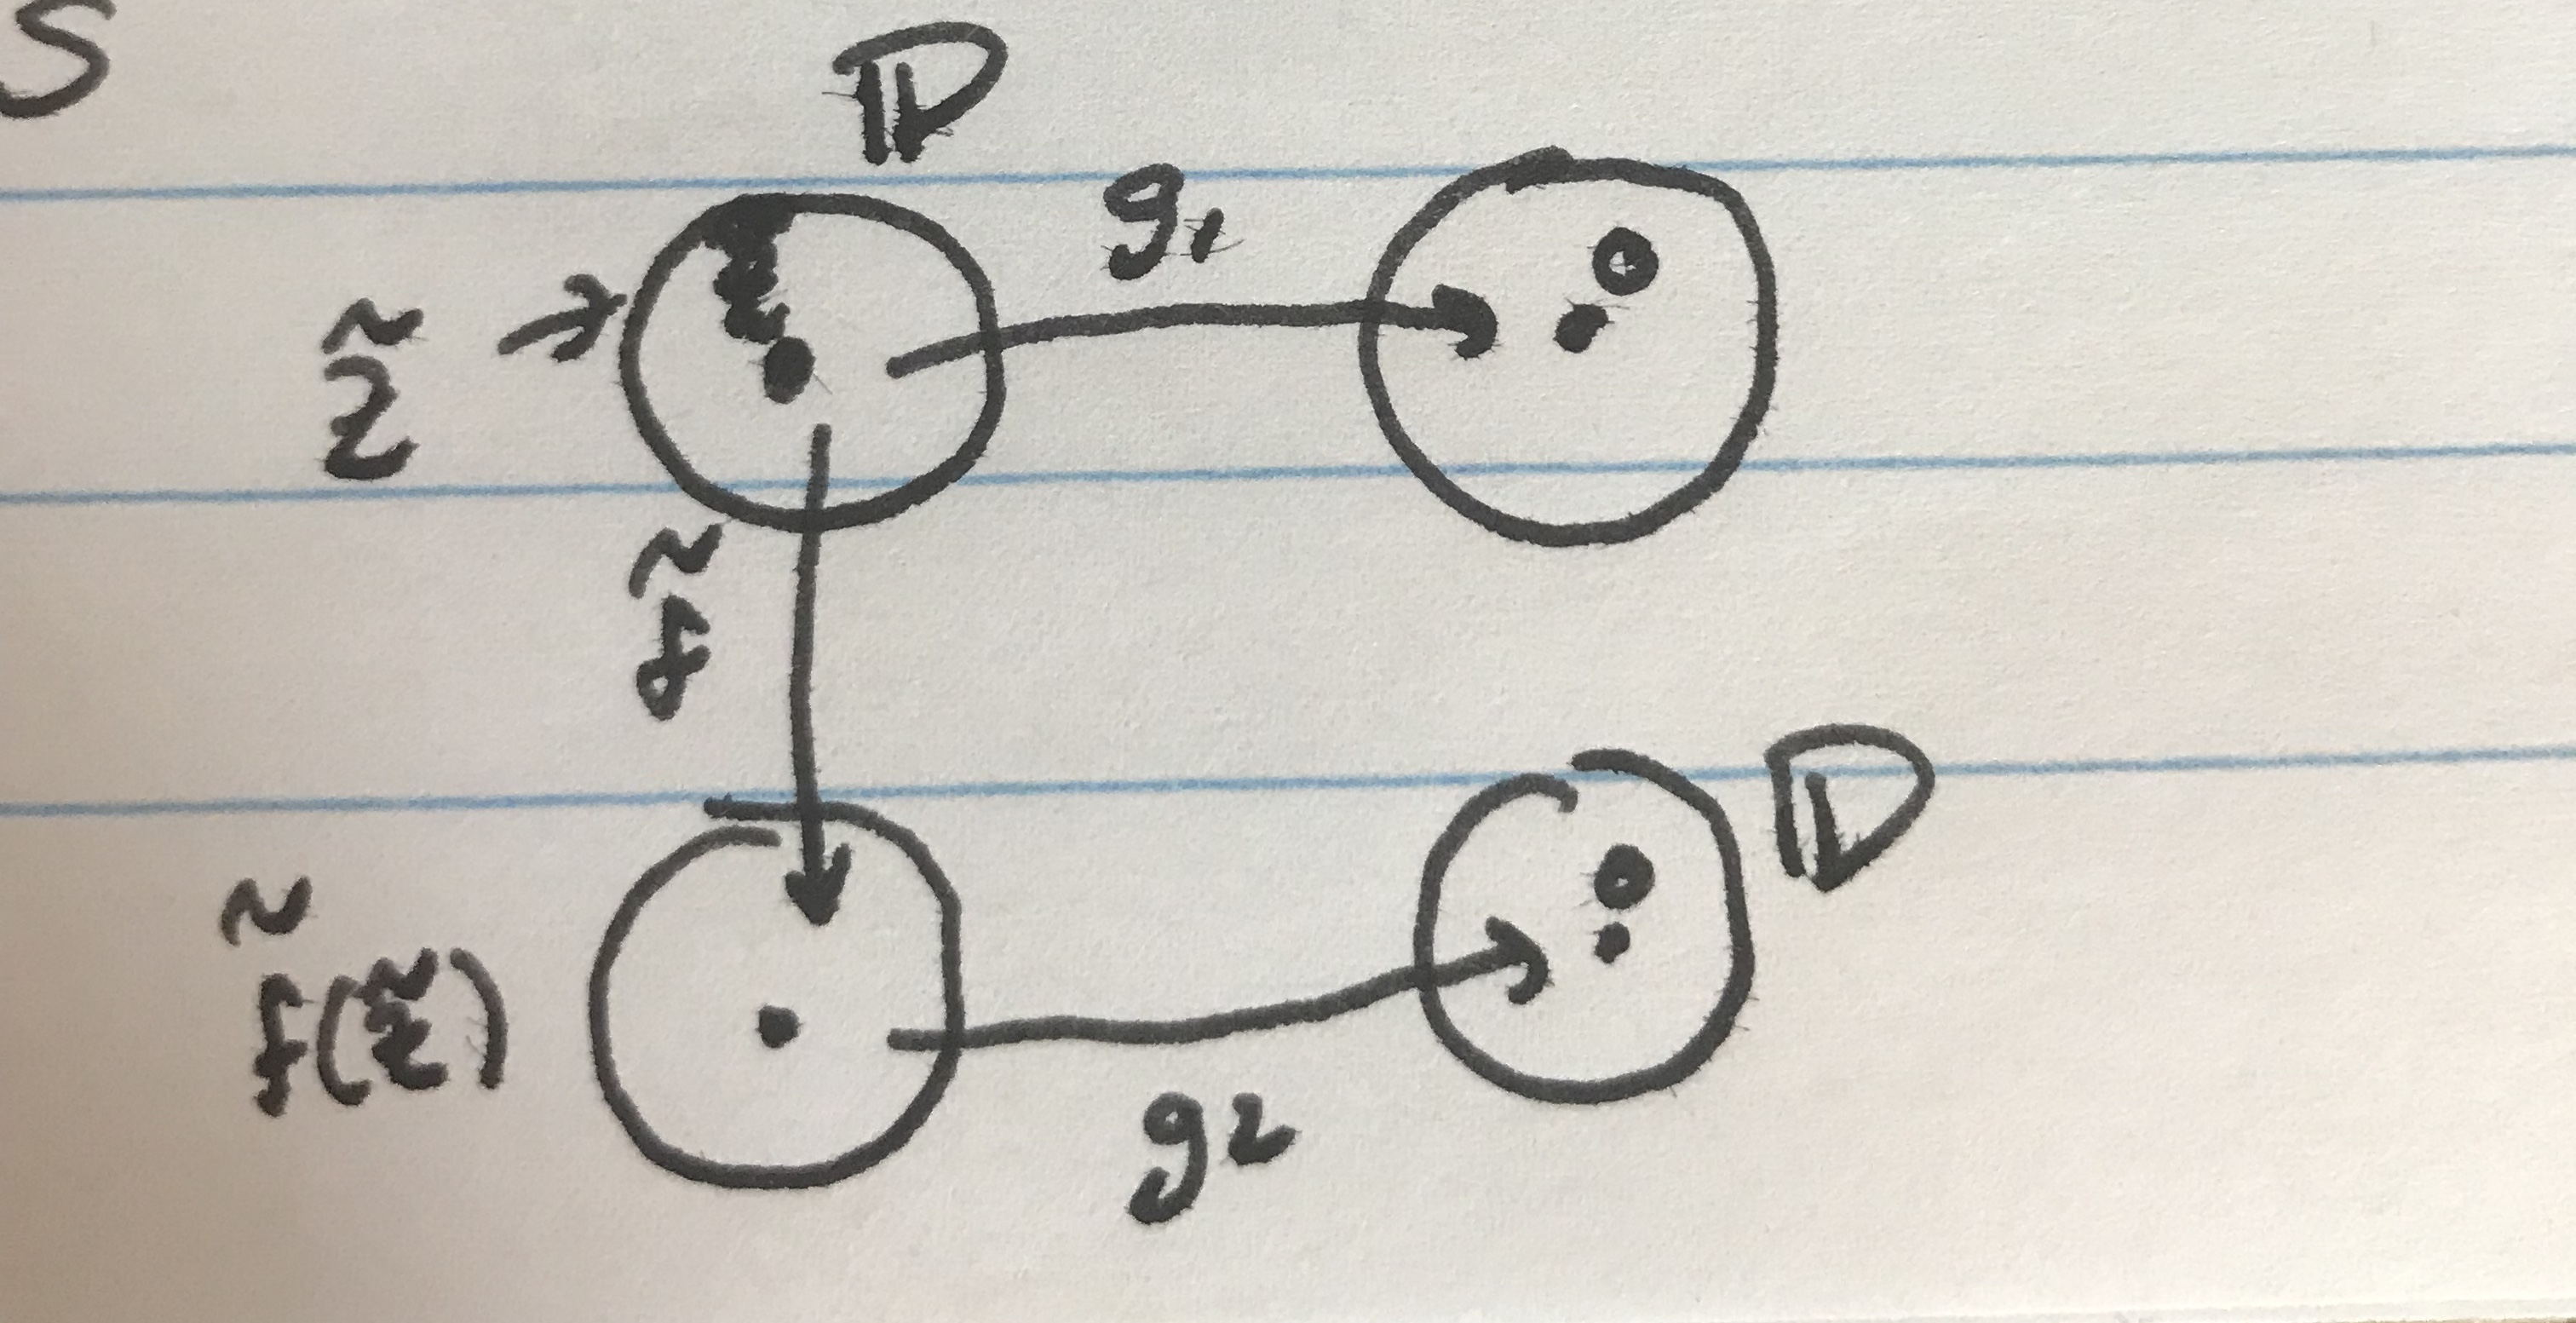
\includegraphics[scale=0.05]{IMG_1016}
        \end{center}
        Then $g = g_2\circ \widetilde{f} \circ g_1^{-1}$ maps $\mathbb{D}\to\mathbb{D}$, $O\to O$.\\

        Hence,
        \[ \norm{d_{g_{E,0}}}\leq 1, \qquad \text{by Schwarz lemma} \]
        where $\norm{d_{g_{E,0}}} = \norm{d\widetilde{f}_{\mathbb{H},\widetilde{z}}}$.\\

        Note: 
        \[ \rho_{\mathbb{D}} = \frac{2|dz|}{1-|z|^2} \simeq 2|dz| \simeq 2\rho_{\mathbb{E}} \]
    \end{proof}

    Examples of Hyperbolic Riemannian surfaces.\\

    1. $X=\mathbb{H},\Gamma = \{z\mapsto \nicefrac{az+b}{cz+d}\}, g(z) = z+1, X = \nicefrac{\mathbb{H}}{z\sim z+1}$.\\
    This forms a cylinder in $\mathbb{H}$ but this is not the same as the cylinder in the Euclidean plane as this Hyperbolic
    one is not locally flat. Recall, $\rho_{\mathbb{H}} = \nicefrac{d|z|}{\eta}$. So, in the Hyperbolic plane, this looks like
    \begin{center}
        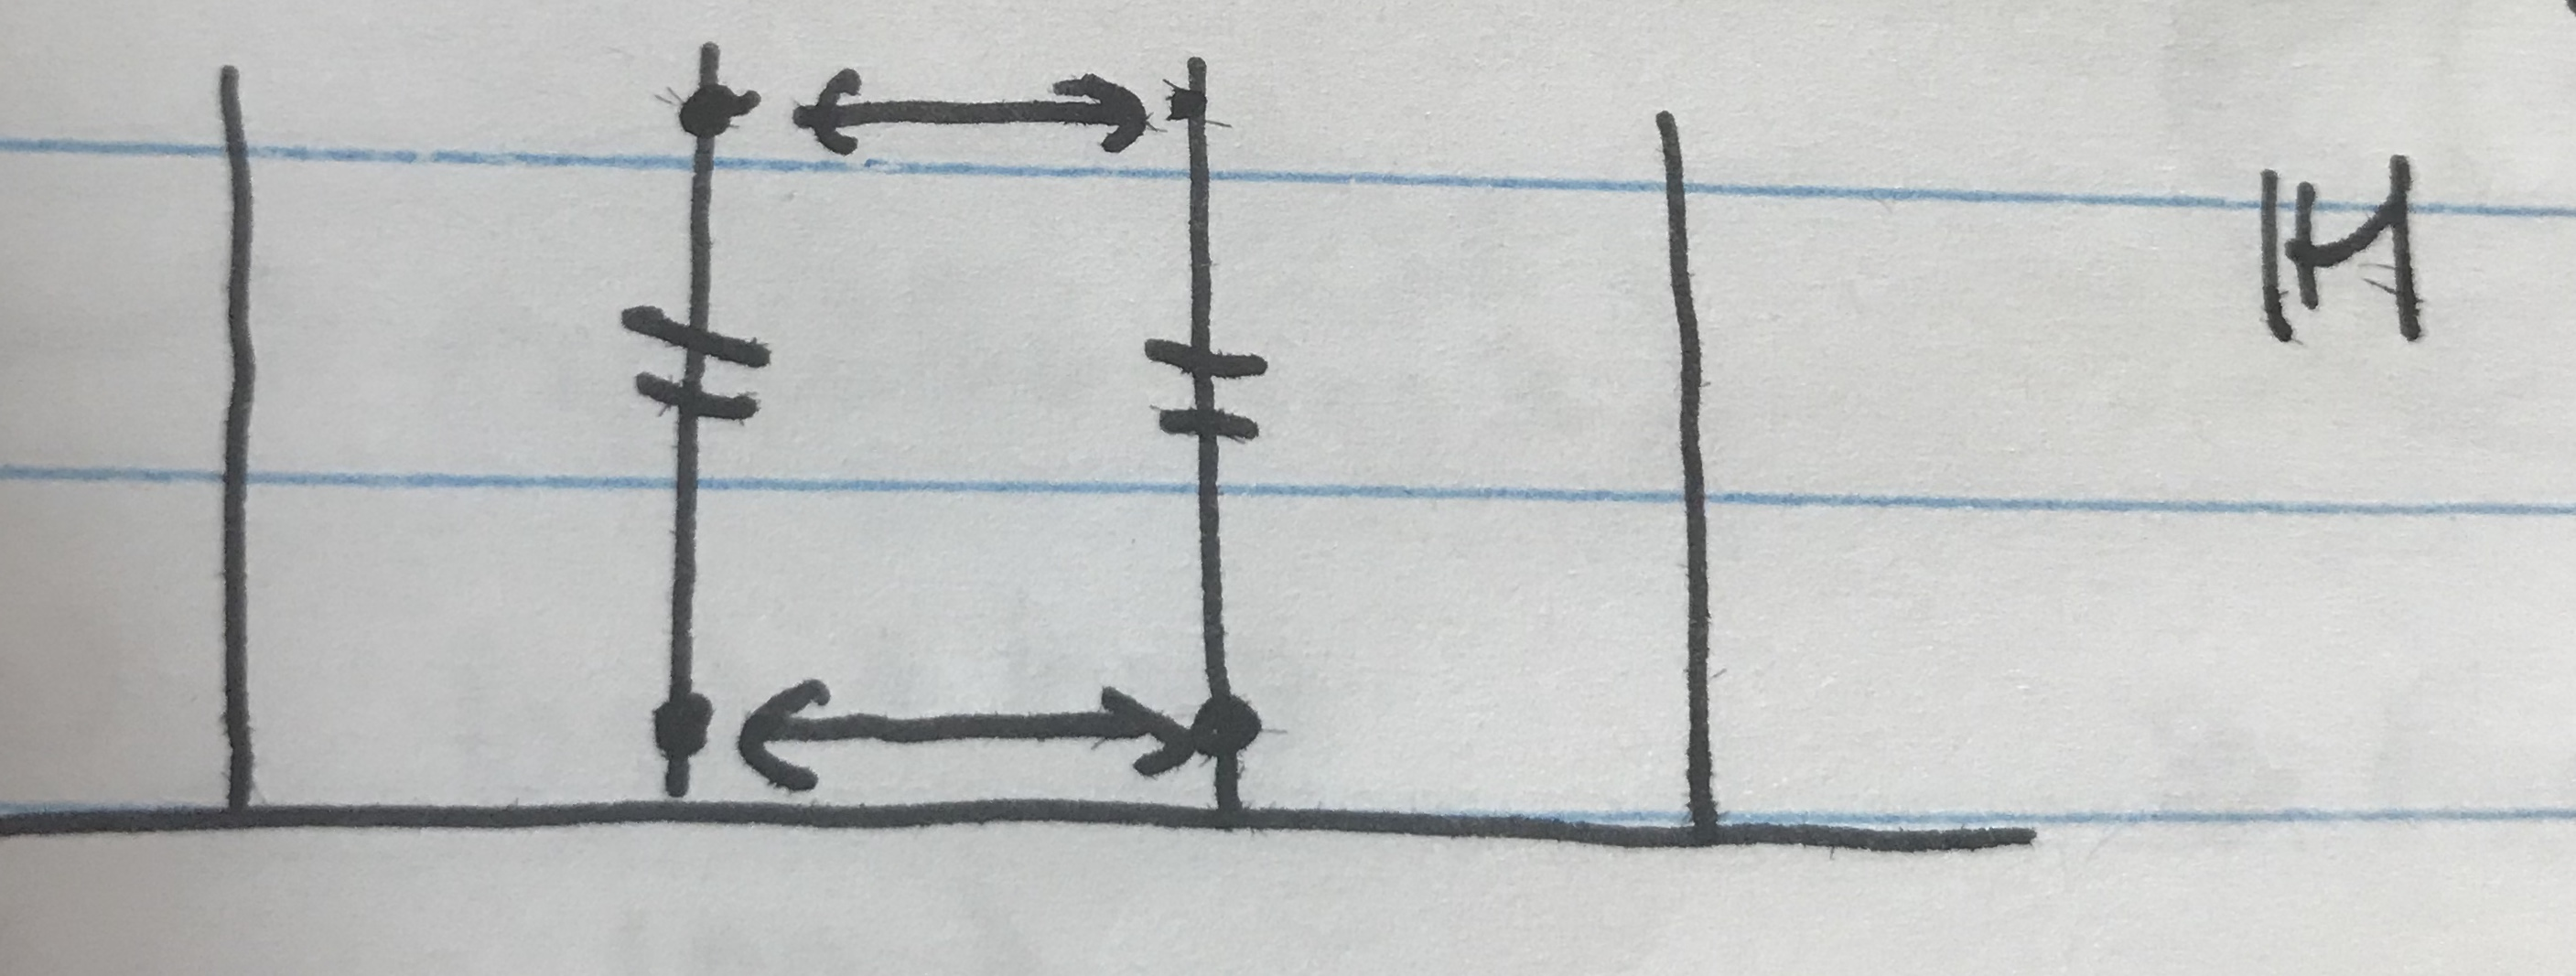
\includegraphics[scale=0.05]{IMG_1017}
    \end{center}
    and can be imagined as:
    \begin{center}
        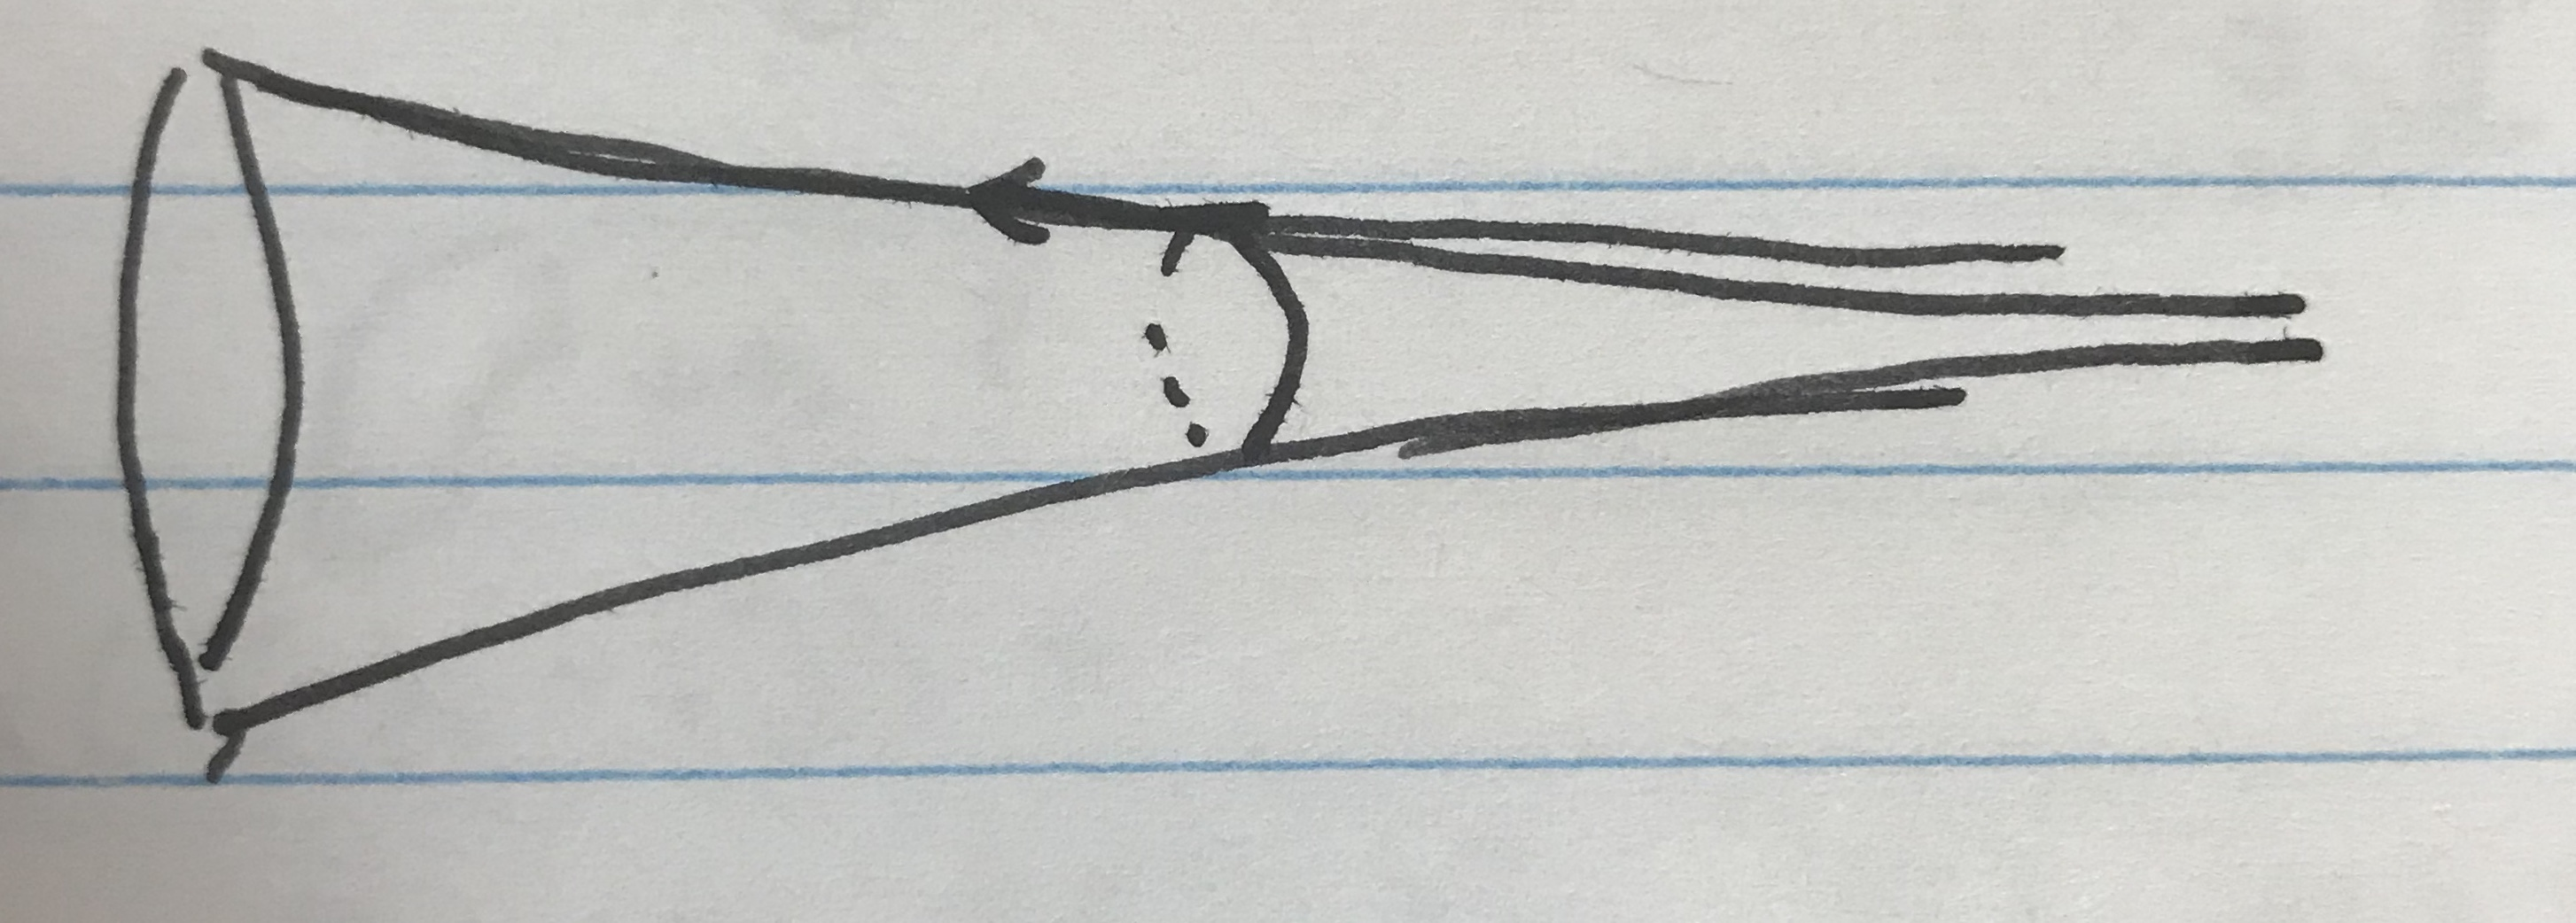
\includegraphics[scale=0.05]{IMG_1018}
    \end{center}
    This is topologically a cylinder but looks very different. Recall, we saw $\nicefrac{\mathbb{C}}{\mathbb{Z}}\simeq\mathbb{C}-\{0\}$
    by exp: $\mathbb{C}\to\mathbb{C}-\{0\}$. This is not Hyperbolic but has similar construction.
    \begin{align*}
        g(z) = e^{2\pi iz},\qquad g:\mathbb{H}\to\mathbb{D}-\{0\} := \mathbb{D}^* \\
        e^{|2\pi iz|} = e^{\text{Re}|2\pi iz} = e^{-\text{Im}(2\pi z)}
    \end{align*}
    So, $\nicefrac{\mathbb{H}}{\mathbb{Z}} \simeq \mathbb{D}^*$.\\

    2. $g(z) = \lambda z, (\lambda > 1), \nicefrac{H}{z\sim\lambda z}$:
    \begin{center}
        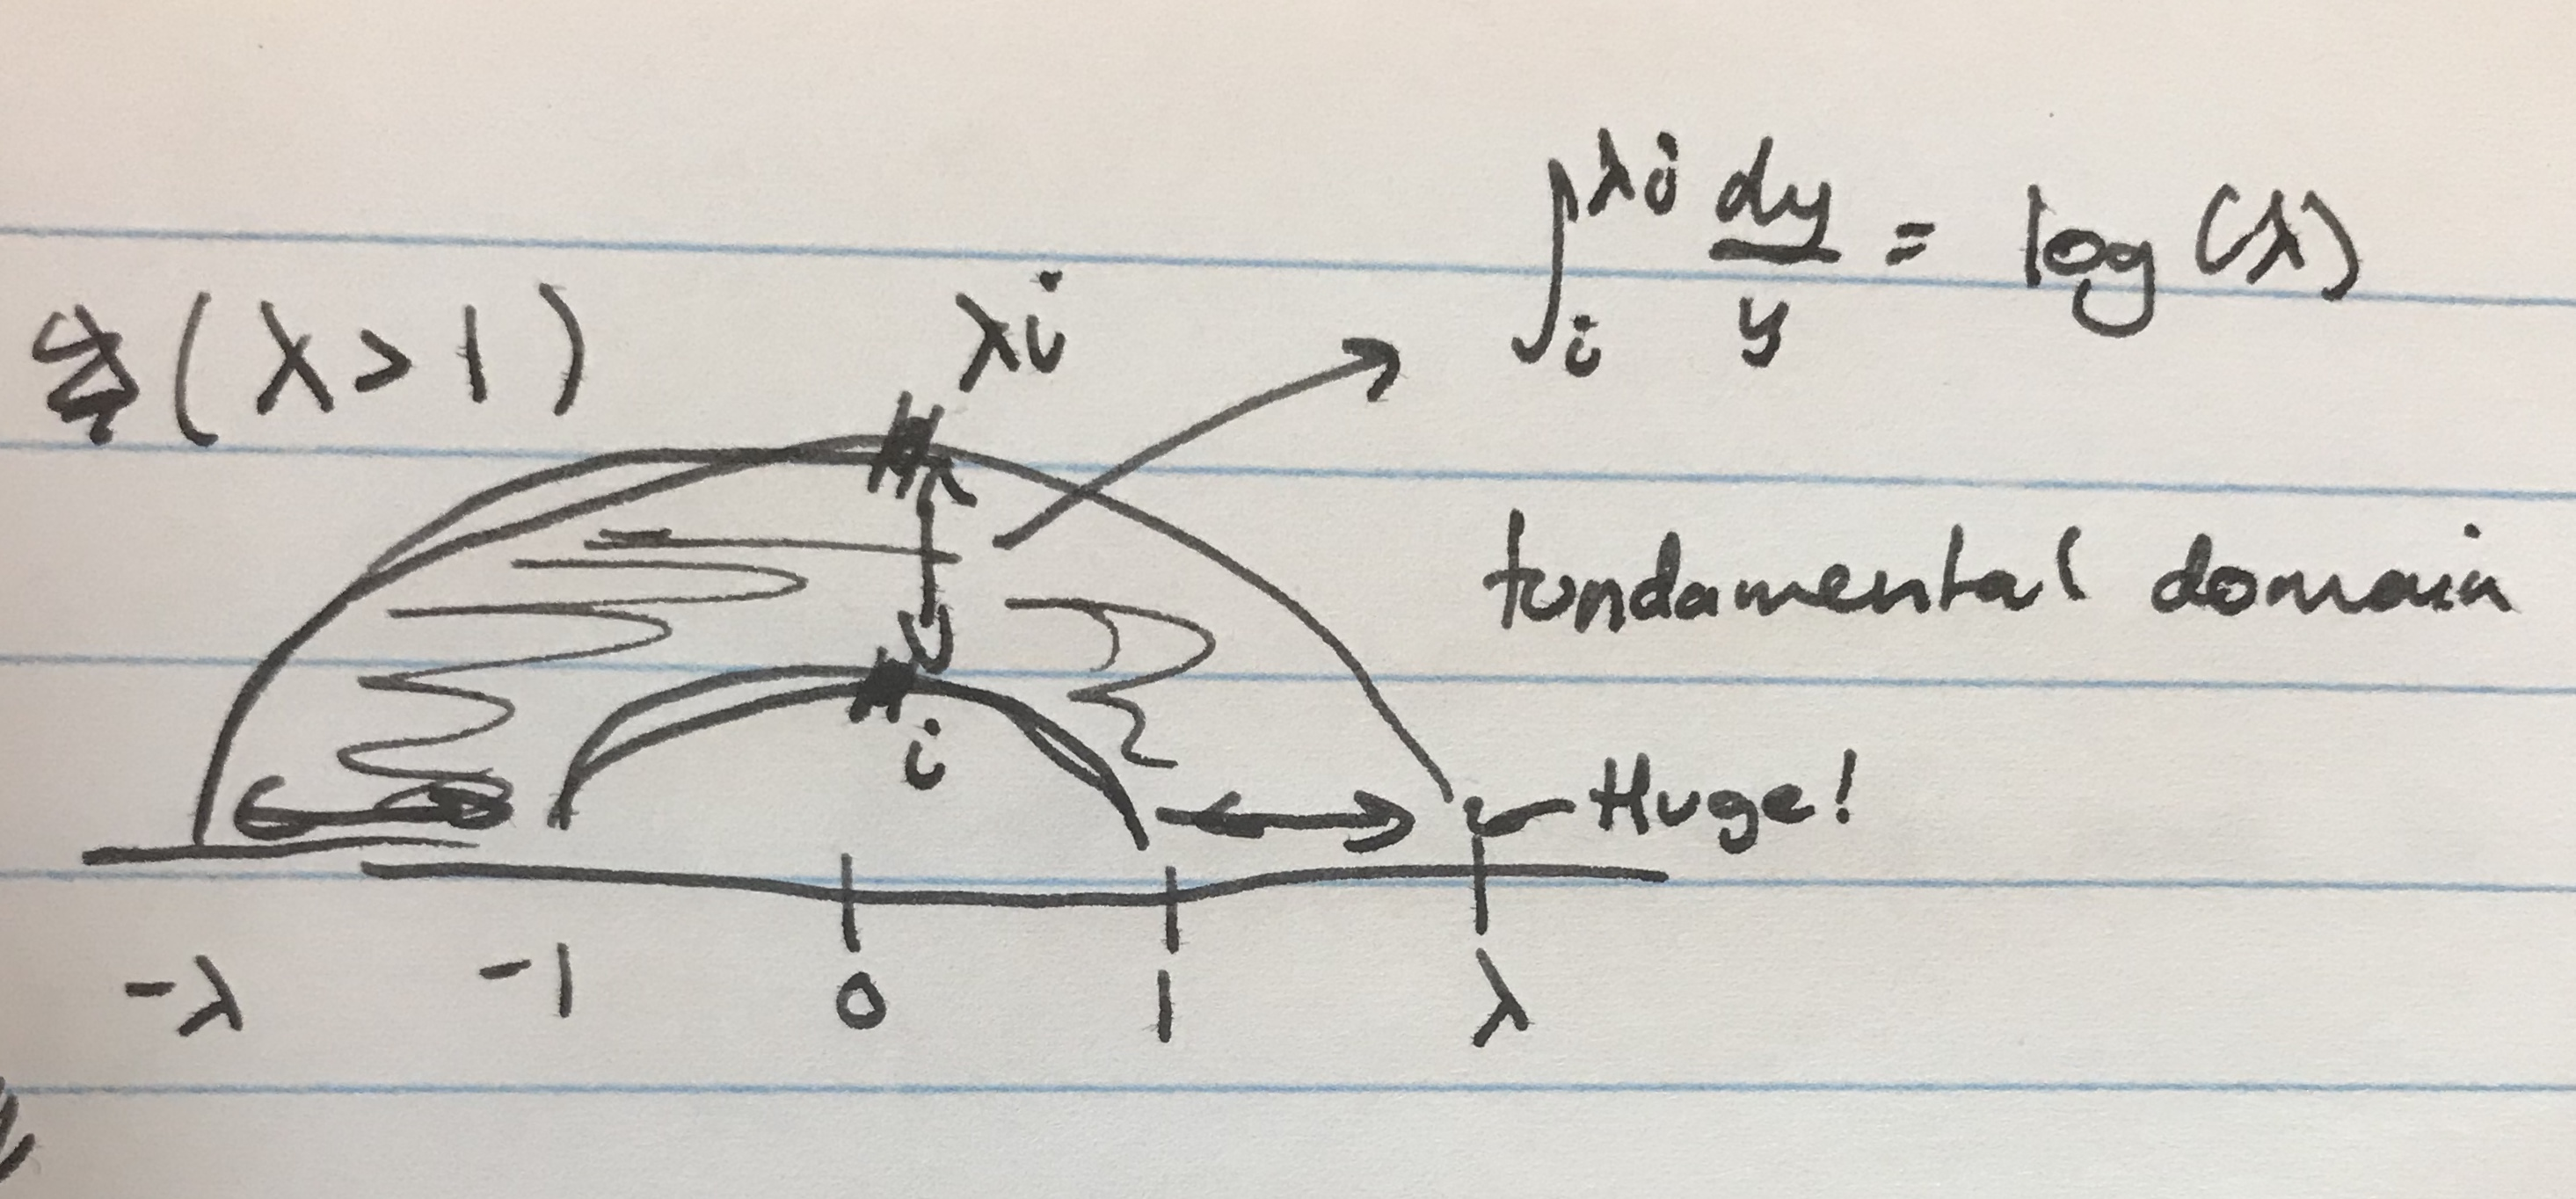
\includegraphics[scale=0.05]{IMG_1019}
    \end{center}
    Note the length of the line segment from $\lambda i$ to $i$ is given by $\int_i^{\lambda i} \frac{dy}{y} = \log{\lambda}$. It
    is also worth noting that length of line segments closer to Im$(z)= 0$ become very big. We can visualise the diagram above as:
    \begin{center}
        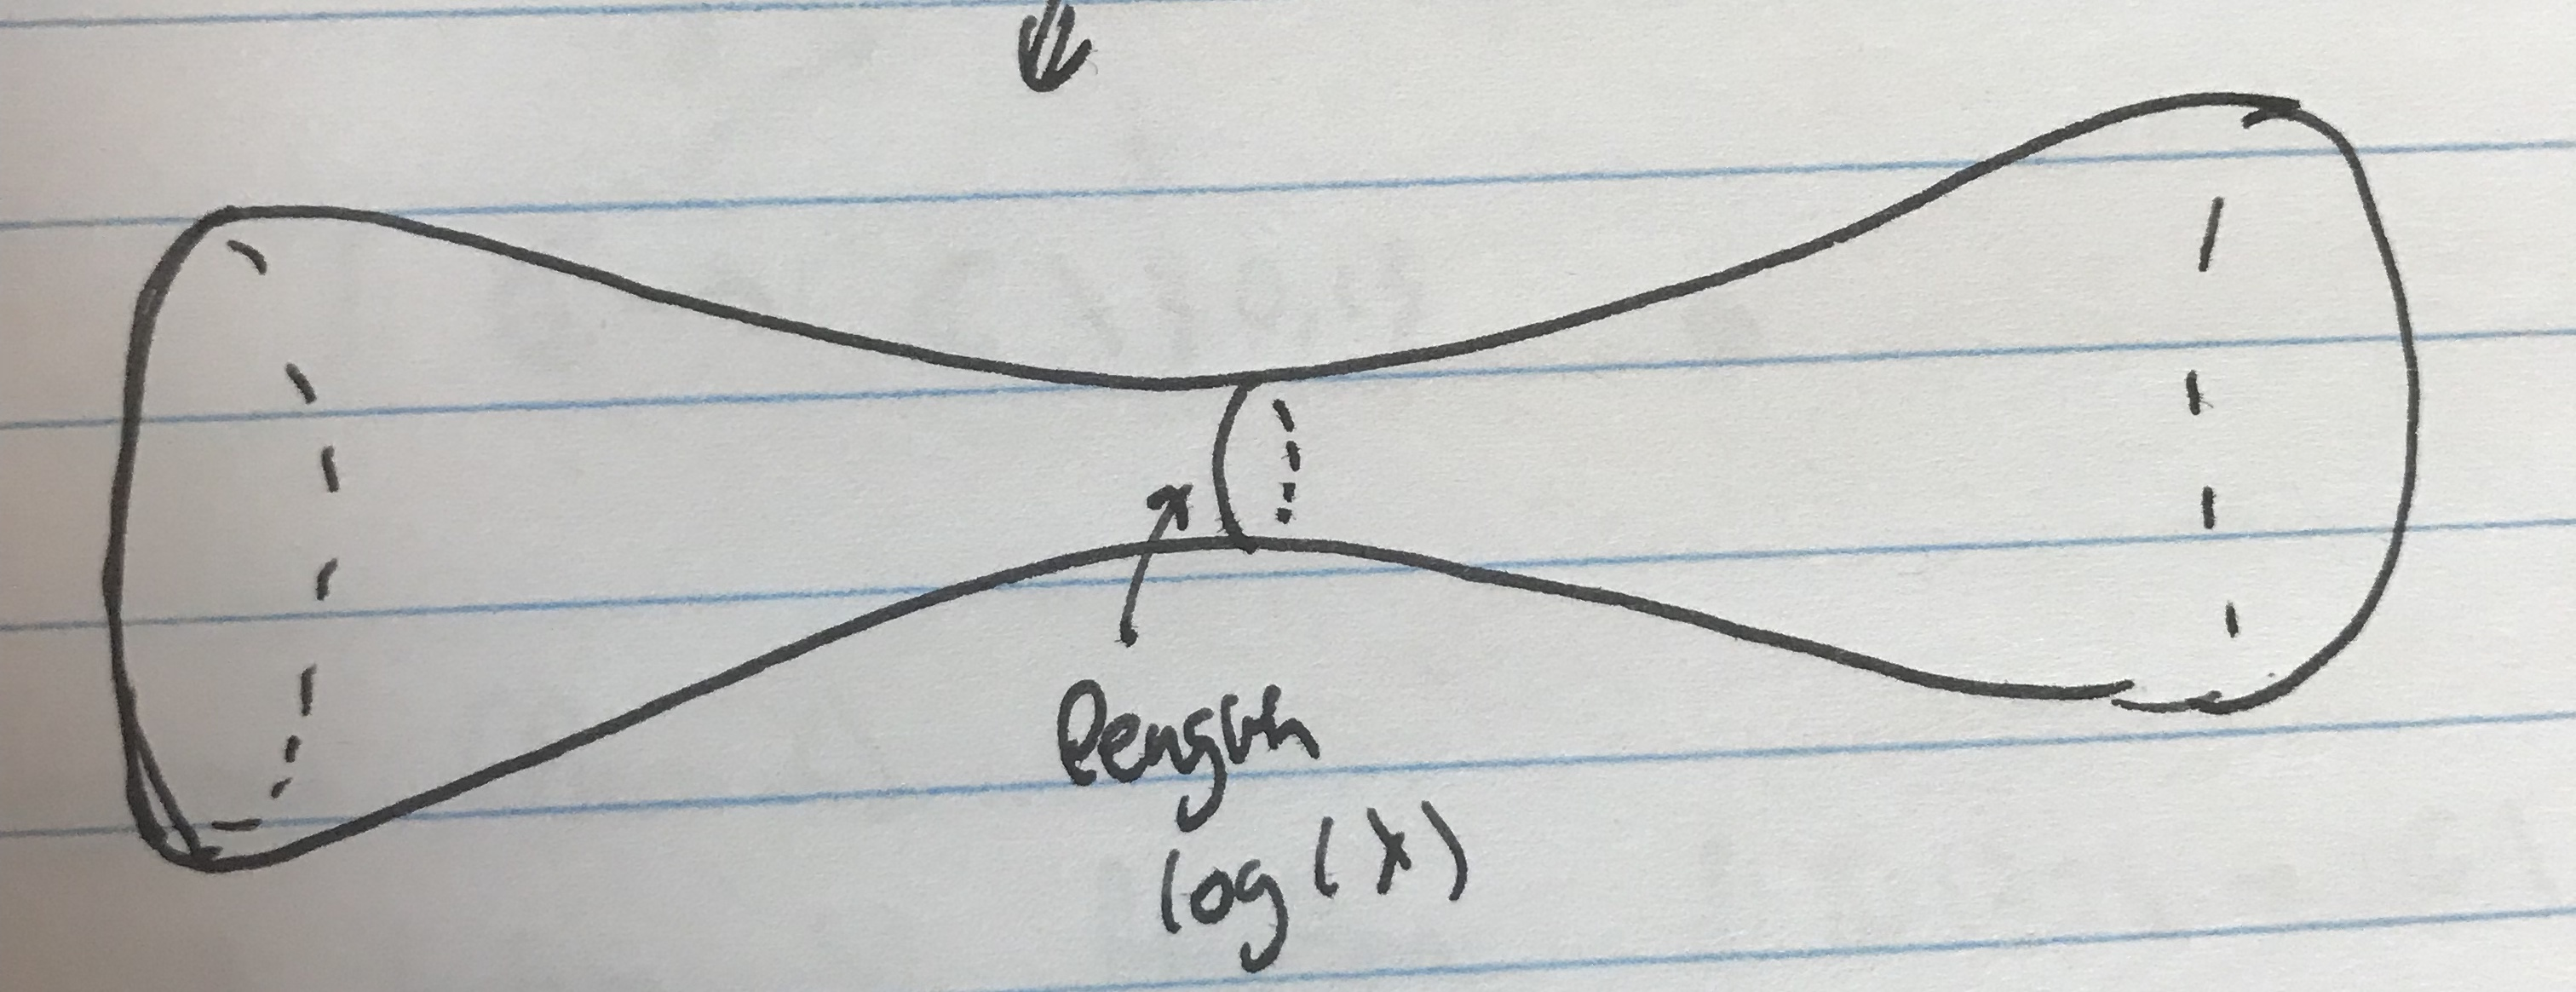
\includegraphics[scale=0.05]{IMG_1020}
    \end{center}
    Where the length of the center in the middle is $\log{\lambda}$.\\

    This is similar to $A_R$, and is actually biholomorphic to this. Note:
    \[ A_R = \{1 < |z| < R\} \]
    \begin{center}
        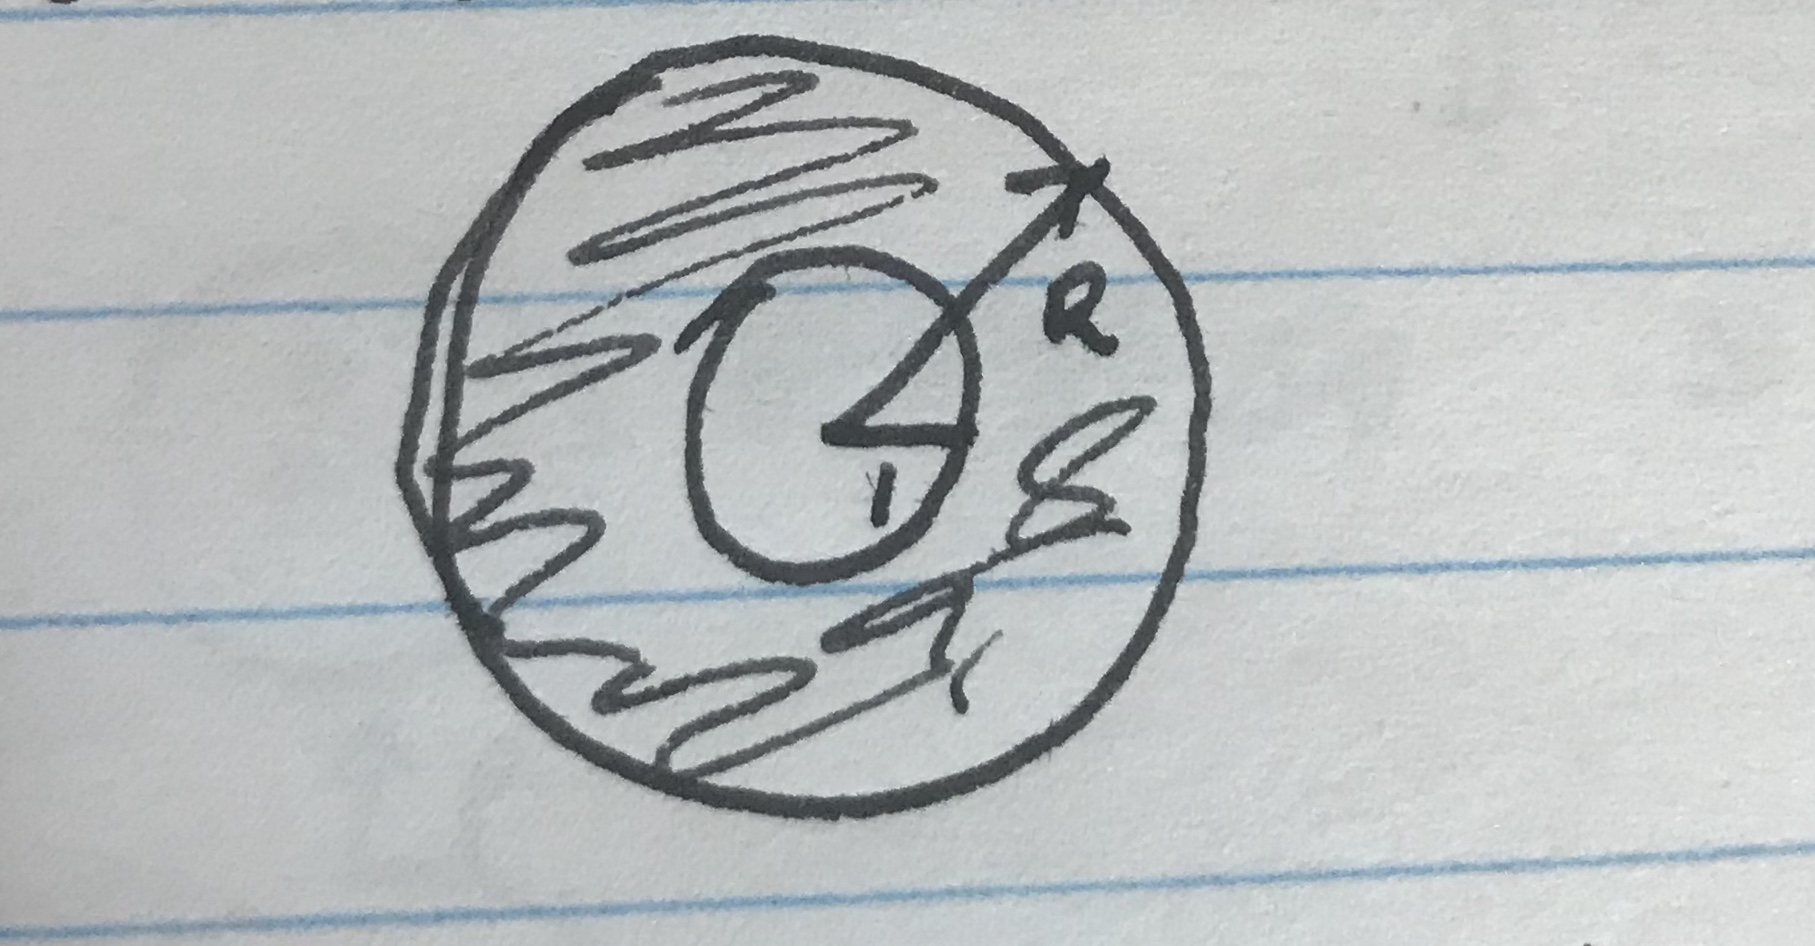
\includegraphics[scale=0.05]{IMG_1021}
    \end{center}
    The map is:
    \[ z\mapsto\;\exp(2\pi i\frac{\log z}{\log \lambda}) \]
    \begin{align*}
        \frac{\log{\lambda z}}{\log{\lambda}} &= \frac{\log{\lambda}} + \log{z}{\log{\lambda}} \\
        &= \frac{\log{z}}{\log{\lambda}}+1
    \end{align*}
    Now, find the image of the map of the right side of the first diagram:
    \begin{align*}
        g_{\lambda}: \frac{\mathbb{H}}{\mathbb{Z}\to\lambda z}\to \mathbb{C} \\
        g_{\lambda}([1,\lambda]) = \{z: |z|=1\} = S^1
    \end{align*}
    Now the question is to see what the other side of the first diagram maps to.
    \begin{align*}
        g_{\lambda}([-\lambda,-1]) &=\\
        z = &-t, t\in[1,\lambda],\nicefrac{\log z}{\log \lambda} = \frac{\log t + \pi i}{\log \lambda} \\
        g_{\lambda}(z) = &\exp(2\pi \frac{\pi i + \log t}{\log \lambda}) = \exp(\frac{-2\pi^2}{\log \lambda})
        \exp(\frac{2\pi i\log t}{\log \lambda})
    \end{align*}
    so that $R = \exp(\nicefrac{2\pi^2}{\log{\lambda}})$.\\

    So, we know what happens at:
    \[ \hat{\mathbb{C}},\mathbb{C} = \hat{\mathbb{C}} - \{\infty\}, \mathbb{C}^* = \hat{\mathbb{C}}-\{0,\infty\} \]
    By exclusion,
    \[ \hat{\mathbb{C}}-\{0,1,\infty\} \]
    is a Hyperbolic Riemann surface.\\

    \begin{corollary}[Little Picard Theorem]
        A holomorphic map from $\mathbb{C}$ to $\mathbb{C}-\{0,1\}$ must be constant.
    \end{corollary}
    \begin{proof}
        \begin{equation*}
            \begin{tikzcd}
                \mathbb{C} \arrow[rr, "\tilde{f}"] \arrow[dr, "f",swap]&  & \mathbb{D}\arrow[dl, ""]\\ 
            & \mathbb{C}-\{0,1\} &
            \end{tikzcd}
        \end{equation*}
    \end{proof}

    \begin{theorem}[Picard]
        A holomorphic function $f:\mathbb{D}-\{0\}\to\mathbb{C}-\{0,1\}$ cannot have an essential singularity $z=0$.
    \end{theorem}
    \begin{proof}
        The diagram here attempts to represent the process in the paragraph below.
        \begin{center}
            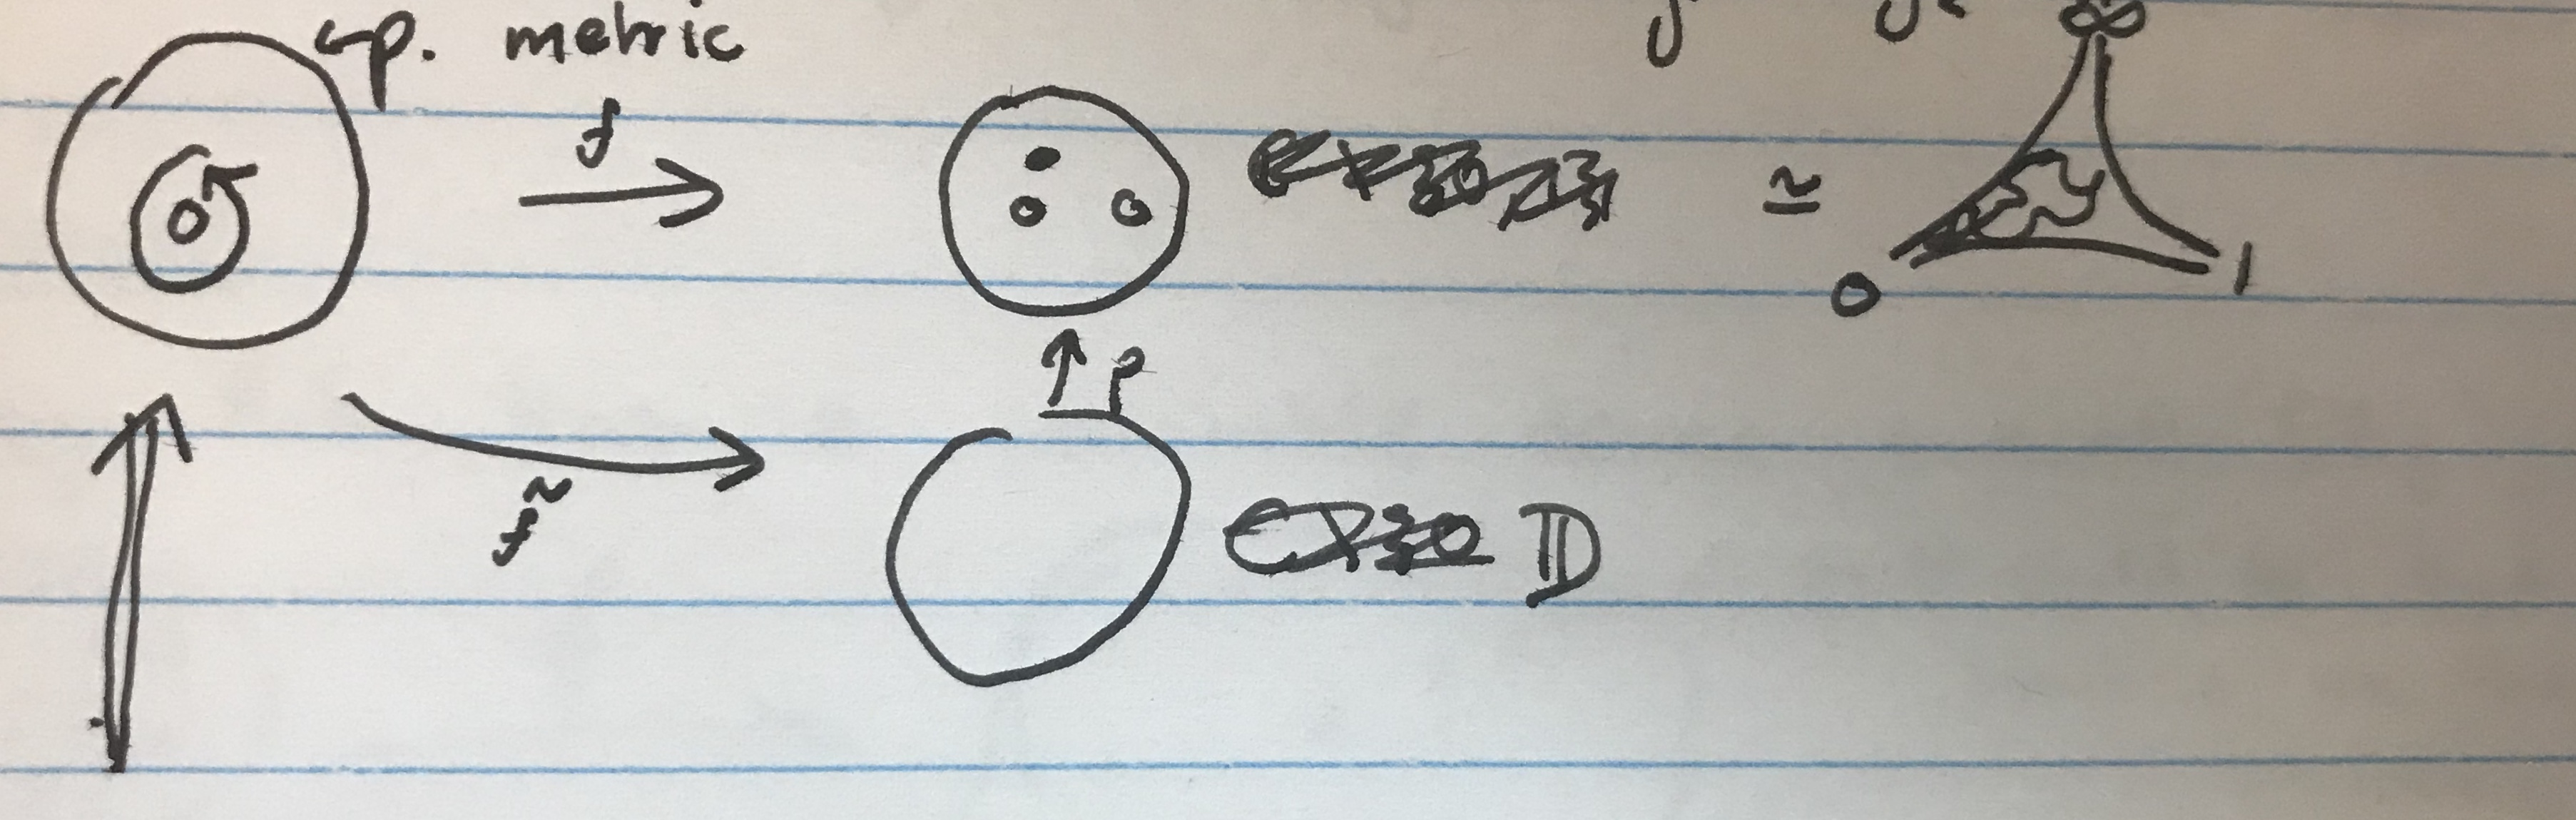
\includegraphics[scale=0.05]{IMG_1023}
        \end{center}
        Pick a loop around 0. Then, the length of the loop must be shorter than the one in the image.\\
        The image must go to 0,1 or $\infty$. Otherwise, the length is too long. If it goes to $\infty$, it has a pole. If not, it
        has a hole that can be filled.
    \end{proof}

    We now begin discussion on Fatou and Julia sets.\\

    \begin{definition}
        A family $\mathfrak{F}$ of holomorphic functions $f:S\to S'$ (with $S'$ compact) is \textbf{normal} if every sequence
        of functions in $\mathfrak{F}$ which converge uniformily on compact sets. Note: the limit of such sequences is holomorphic.
    \end{definition}

    \begin{theorem}[Montel's theorem]
        If $S$ is a Riemann surface and $S'\subseteq\hat{\mathbb{C}}-\{0,1,\infty\}$, then every family of holomorphic functions
        $f: S\to S'$ is normal.
    \end{theorem}

    This is somewhat similar to Arzelà-Ascoli theorem.

    \begin{remark}
        A limit $g$ of such convergent family need not take values in $S'$.
    \end{remark}

    \begin{proof}
        Recall, any Riemann surface has a countable dense subset $(z_j)_{j\in\mathbb{N}}\subseteq S$,
        \begin{center}
            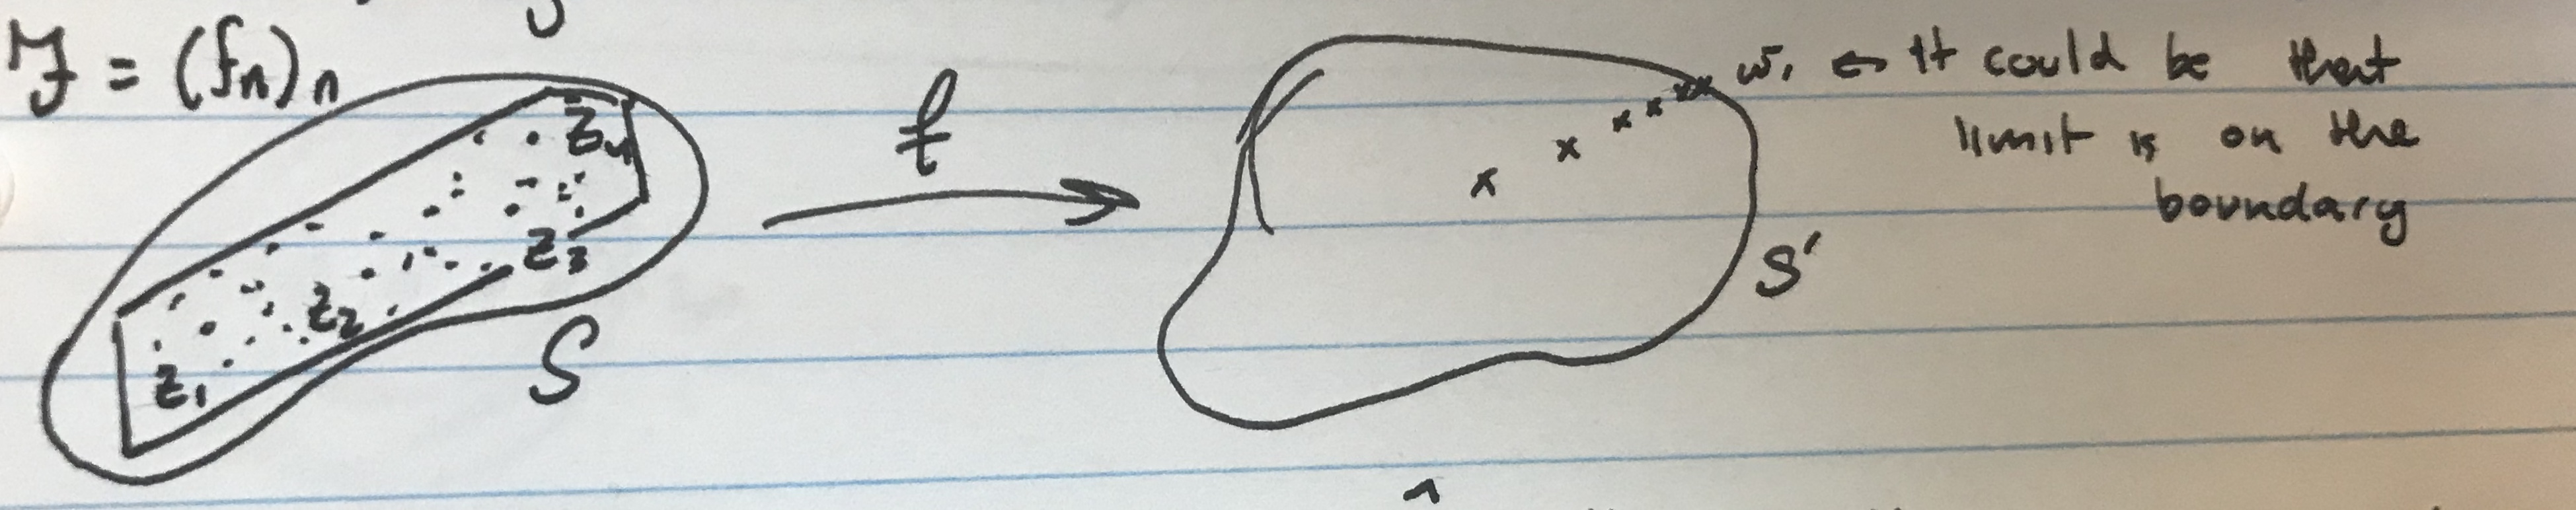
\includegraphics[scale=0.05]{IMG_1024}
        \end{center}
        For each $j$, $(f_n(z_j))_{n\in\mathbb{N}}\subseteq\hat{\mathbb{C}}$. Hence, there is a subsequence $f_{n_1}(z_1)\to w_1\in
        \overline{S'}$.\\

        Now, consider $(f_{n_2}(z_2))_{n\in\mathbb{N}}\subseteq\hat{\mathbb{C}}$, hence there is a subsequence 
        $f_{n,2}(z_2)\to w_2\in\hat{\mathbb{C}}$. Hence by taking diagonal, there is a subsequence $g_n\in\mathfrak{F}$, such that
        $g_n(z_j) \to w_j$ for all $j$ as $n\to\infty$. We then have two cases, either $w_1\in S'$ or $w_1\in\partial{S'}-S'$.

        Case 1: $w_1\in S'$.\\
        Pick a compact set $K\subseteq S$ and $\epsilon>0$. Choose $z_1,\hdots,z_n\in K$ such that
        \[ K \subseteq \cup_{i=1}^N B(z_i,\epsilon) \]
        By construction of $(g_n)$, there exists $n_0$ such that for all $m,n > n_0$,
        \[ d_{S'}(g_n(z_i),g_m(z_i)) < \epsilon \]
        for all $i = 1,\hdots,N$ where $d_{S'}$ is the Poincaré metric. Hence, if $z\in K$, there exists $i$ such that
        \[ d_{S'}(z,z_i)<\epsilon \]
        and
        \begin{align*}
            d_{S'}(g_n(z),g_m(z)) &\leq d_{S'}(g_n(z),g_n(z_i)) + d_{S'}(g_n(z_i),g_m(z_i)) + d_{S'}(g_m(z_i),g_m(z)) \\
            &\leq d_{S'}(z,z_i) + d_{S'}(z_i,z) \leq 3\epsilon
        \end{align*}

        Case 2: $w_1\in \partial{S'}{S'}$.\\
        $g_n(z_1)\to w_1\in \partial{S'}{S'}$. Pick $K\subseteq S$ compact, then there exists $\mathcal{C}>0$ such that
        $d_{S'}(g_n(z),g_n(z_1)) < \mathcal{C}$ for all $z\in K$, for all $n$. Hence, for each $z\in K$, then
        \[ \lim_{n\to\infty} g_n(z) = w_1 \]
    \end{proof}

    \begin{lemma}
        If $S'$ is hyperbolic $\subseteq \hat{\mathbb{C}}$ and $z_k\to z_{\infty}\in \partial{S'}$, then for each $\epsilon>0$
        \[ N_{\rho_{S'}}(z_k,\epsilon) \to z_{\infty} \]
        as $k\to\infty$.
    \end{lemma}

\end{document}
